%% Author_tex.tex
%% V1.0
%% 2016/09/02
%% developed by Techset
%%
%% This file describes the coding for cta-author.cls

\documentclass{cta-author}%%%%where cta-author is the template name

\newtheorem{theorem}{Theorem}{}
\newtheorem{corollary}{Corollary}{}
\newtheorem{remark}{Remark}{}

%%%%%%Begin MyPackages%%
\usepackage[utf8]{inputenc}
\usepackage[T1]{fontenc}
\usepackage{framed}
\usepackage{graphicx}
\usepackage{multirow}
\usepackage{booktabs}
\usepackage{color}
\usepackage{tabulary}
\usepackage{enumitem}
	\setlist[itemize]{leftmargin=5.5mm}

%\usepackage{hyperref}
%\usepackage{url}
\usepackage[hyphens]{url}
\usepackage[hidelinks]{hyperref}
\hypersetup{breaklinks=true}
\urlstyle{same}

\usepackage{natbib}
\setcitestyle{square}

\usepackage{soul}
\usepackage{rotating}
\usepackage{lscape}
\usepackage{caption}
\usepackage[title]{appendix}
\usepackage{ulem}
\usepackage{placeins}
\usepackage{balance}
\usepackage[autostyle, english = american]{csquotes}
\MakeOuterQuote{"}

\usepackage[draft]{changes}
\definechangesauthor[name=version2, color=blue]{v2}
\definechangesauthor[name=version3, color=red]{v3}
\definechangesauthor[name=version3, color=brown]{v4}

%%%%%%end MyPackages%%%%

%% Para arreglar las viñetas

\setitemize{label={\raisebox{0pt}{\normalsize\textbullet}}, labelindent=0em,labelsep=1em,leftmargin=*}

%% Hay otros cambios en el .cls

\begin{document}

\supertitle{Submission Template for IET Research Journal Papers}

\title{Investigation of the activities performed by experimental researchers in a software engineering lab using an ethnographic methodology}

\author{\au{Efraín R. Fonseca C.$^{1\corr}$}, \au{Oscar Dieste$^{2}$}, \au{Natalia Juristo$^{2}$}}

\address{\add{1}{Departamento de Ciencias de la Computación, Universidad de las Fuerzas Armadas - ESPE, Av. General Rumiñahui s/n y Ambato, Quito, Ecuador}
\add{2}{Departamento de Lenguajes y Sistemas Informáticos e Ingeniería de Software, Universidad Politécnica de Madrid, Calle de los Ciruelos, 28660, Madrid, España}
%\add{3}{Third Department, Third University, Address, Country Name}
%\add{4}{Current affiliation: Fourth Department, Fourth University, Address, Country Name}
\email{erfonseca@espe.edu.ec}}

\begin{abstract}
\textbf{Context:} Replication is complex in Experimental Software Engineering (ESE). Replication packages and families of experiments have been applied with limited success. We wonder whether the problems are due to formal issues, e.g., under-specification, miscommunication, etc., or intrinsic reasons, i.e., the researchers' needs are not fulfilled by the existing replication procedures.
\textbf{Objective:} Find out how ESE researchers conduct experiments in practice.
\textbf{Method:} Ethnographical study with an experimental research group.
\textbf{Results:} We have created conceptual and process models representing how experimentation, replication, and synthesis are conducted in the target research group. These models fit the mainstream procedures and terminology at a high level but depart at lower, specialized levels. The experimental process carried out in the group differs from folk knowledge and textbooks in (1) the number and diversity of activities, (2) the existence of different roles, (3) the granularity of the concepts, and (4) the viewpoints that different sub-areas or families of experiments have about the experimental process.
\textbf{Conclusions:} The differences between the actual lab processes vs. the idealized versions probably harm knowledge transfer and make replication harder. We will conduct further research with more research groups, e.g., using a survey, to explore whether our findings have general applicability.
\end{abstract}

\maketitle

%%%%%%% Begin Content %%%%%%%
\section{Introduction}\label{sec-introduction}
Replication is troublesome in general \cite{Klein-2018-many}, particularly in the social and life sciences \cite{Pashler-2012-perspectives,Baker-2016-lid-reproducibility}. In Empirical Software Engineering (ESE%
\footnote{\added[id=v4]{The acronyms used throughout the paper are listed in Table~\ref{tab:acronyms} in the appendix.}}%
)\added[id=v3]{, there is a consensus that replications are important \cite{shepperd2018role}, but} the number of replications is small \cite{Bezerra-2015-Replication-SE-U-SMS} and the rate of confirmation of previous results is limited \cite{Jorgensen-2016-Incorrects-Results-SEE}.

Several reasons prevent replication. They have discussed elsewhere, e.g., \cite{Miller-2005-replicating-SE-experiments,Demagalhaes-2015-replications-SE,cockburn2020threats,mahmood2018reproducibility,dos2022investigating}. In this paper, we focus on a potential cause that, to our knowledge, has not been explored so far: How ESE researchers \textit{really} experiment. 

Anecdotic evidence such as conversations with other researchers, review of articles, and direct observation suggests that researchers follow \textit{in practice} different \textit{experimental processes}, i.e., the different activities that ESE researchers perform to conduct experiments. Experiment reports look relatively uniform due to the existence of reporting guidelines \cite{Carver-2010-guidelines-replication-SE,Jedlitschka-2008-reporting-experiments-SE}, but the underlying data generation processes vary.

This paper aims to \replaced[id=v2]{investigate}{determine} \textbf{how experimental researchers conduct experiments in practice}. \added[id=v2]{We intend to find out how experimental researchers plan, execute, analyze, and report their investigations and what concepts, protocols, and processes they use.}

We applied an ethnographic method \cite{Sharp-2016-Ethnographic-Studies-ESE,zhang2019ethnographic} within an experienced experimental research group. We observed the researchers in their lab for two years. We created conceptual and process models to represent the concepts they use and the activities they perform daily. These models fit the community's procedures and terminology at a high level. Still, the models show particularities at lower levels: (1) The number and diversity of activities, (2) the existence of different roles, (3) the granularity of the concepts used by the roles, and (4) the viewpoints that different subareas or families of experiments have about the overall process.

The contributions of this paper are:

\begin{itemize}
  \item Identifying activities that depart from or are not described in mainstream experimentation procedures. 
  \item Characterizing roles, i.e., groups of experimental activities performed by the same person, in ESE research.
  \item Evidence of the existence of tacit knowledge in ESE, which, in turn, leads to discrepancies between experimentation protocols and actual practice.
  \item Conceptual and process models that represent how experimentation is conducted \textit{in practice} in an experimental research group.
\end{itemize}

Finally, we wish to open a discussion in the ESE community: 
\begin{itemize}
  \item Should those differential characteristics in experimentation in software engineering be disregarded as inherently contextual?
  \item  \textbf{Alternatively}: Are they more common than they may seem, so they should be further investigated and eventually integrated into mainstream practice?
\end{itemize}

The remainder of the article is structured as follows: Section \ref{sec-research-method} describes the research method. Section \ref{sec-reseach-execution} reports the stages of the ethnographic research and the observations made. Section \ref{sec-results} reports the concept and process models. Section \ref{sec-related} discusses the results and the connections with the existing literature. Section \ref{sec-threats} details the threats to validity and the related mitigation strategies. Finally, in Section \ref{sec-conclusions}, we present the conclusions and future work.
\section{Research Method}\label{sec-research-method}
Ethnography is a \textit{participant observation} method. It does not interfere (beyond the ethnographic researchers' presence) with the observed ESE researchers' "life" \cite{Sharp-2016-Ethnographic-Studies-ESE}. Ethnographic researchers adopt "the ESE researchers' point of view" to better understand the reason for their actions \cite[pp. 55-56]{Outhwaite-2007-sage}. Thus, the biases and misperceptions that ESE researchers might have about themselves can be detected. Ethnography also captures the rich context that surrounds ESE researchers.

Ethnography identifies details that are ignored by or in other methods. The disadvantage is the time required for learning \cite{Sharp-2016-Ethnographic-Studies-ESE}. Thus, we opted to study a single experimental research group over a long period instead of working halfway with several experimental research groups over shorter periods. This decision was also motivated by the challenge of finding several open-minded experimental research groups willing to participate in this research. We selected a representative, i.e., respected and well-known, research group to guarantee (to the extent possible) the reliability of the results, their validity, and the findings' scientific significance \cite{sjoberg-2007-future-empical-methods}.

We followed Runenson et al.'s case study guidelines \cite{Runenson-2012-case-study-SE} wherever they apply to ethnographical studies. Our research protocol is organized along three axes:

\begin{itemize}
	\item \textbf{Context selection}, i.e., choose the experimental research group that facilitates the research in the best possible condition.
    \item \textbf{Data collection procedures}.
    \item \textbf{Data analysis procedures}.
\end{itemize}

To avoid confusion, from this point on, we will refer to the "ESE researchers" with whom we interact during the investigation as "the experimenters". We will talk about ourselves, the authors, as "the researchers". We, authors/researchers, play two different roles in the investigation:

\begin{itemize}
\item \textbf{Efra\'in R. Fonseca C.} and Edison G. Espinosa conducted the ethnographic study as part of their Ph.D. Edison G. Espinosa abandoned the ethnographic study early (during the investigation reported in Section~\ref{replication}) and changed the orientation of his Ph.D. This is the reason he is not authoring this paper. The personal opinions poured in Section~\ref{sec-reseach-execution} belong to these two researchers, particularly Efra\'in R. Fonseca C.
\item \textbf{Oscar Dieste} and \textbf{Natalia Juristo} supervised the investigation. Their views and opinions are not reflected in this manuscript.
\end{itemize}

\subsection{Context selection}
We have considered an experimental research group as "representative," i.e., a reliable source of information when it fulfills the following selection criteria:

\begin{itemize}
	\item The experimental research group has extensive experience in ESE research.
	\item The ESE community recognizes the experimenters as specialists in their areas.
	\item The group has many publications in journals of repute and internal documentation, i.e., the group has a verifiable track record.
\item One of the main drivers of this research is to explore the connection between replication and lab practices. We positively value that the experimental research group conducts replications or families of experiments.
\end{itemize}

Based on these criteria, we selected an experimental research group with more than 20 years of experience in experimentation in SE. The experimenters have a long track record of publication in journals and conferences of repute. The group has focused on replications and families of experiments since they consider that isolated experiments do not contribute significantly to scientific knowledge. The manuscript conceals the group's identity but is disclosed in the raw data repository (see Section \ref{sub-sec-research-documentaition}).

\subsection{Data collection procedures}\label{subsec-data-collection}

The information sources within the experimental research group under study (RGUS) are:

\begin{itemize}

	\item Experimenters' knowledge.
	
	\item General and specific literature, e.g., the book \textquotedblleft Experimentation in Software Engineering\textquotedblright~\cite{Wohlin-2012-experimentatio-SE}.
	
	\item General and specific experimental materials, e.g., experimental designs.
	
	\item Periodic and/or \textit{ad-hoc} activities carried out, e.g., experimental planning.
	
\end{itemize}

Ethnography information gathering is characterized by being cyclical, iterative, and incremental. The data acquisition process was based on a taxonomy of information-gathering techniques, categorized according to the level of contact with the primary source of information. Such a taxonomy proposes three levels of information gathering: direct participation with the source (level 1), indirect participation with the source (level 2), and study of the experiment material without the participation of the source (level 3) \cite{Lethbridge-2005-data-collection-techniques-SE}. Table \ref{tbl-tecnica-fuente} describes the information-gathering techniques and instruments and the corresponding information sources to which they can be applied.

\begin{table}
	\small
	\centering
	\caption{Techniques and tools for information acquisition, by source}
	\label{tbl-tecnica-fuente}
	\begin{tabular}{|p{2cm}|p{2.5cm}|p{3cm}|}
	\hline
	\textbf{Source} & \textbf{Technique} & \textbf{Instruments}\\
	\hline
	\multirow{14}{50 pt}{Experimenters knowledge} & Interviews & Video camera, paper, pencil\\
	\cmidrule{2-2}\cmidrule{3-3}
	& Focus groups & Video camera, blackboard, cardboard, board markers, chalkboard eraser, etc.\\
	\cmidrule{2-2}\cmidrule{3-3}
	& Process modeling & Video camera, paper, pencil\\
	\cmidrule{2-2}\cmidrule{3-3}
	& Instrumental systems & Email, videoconferences, internet\\
	\cmidrule{2-2}\cmidrule{3-3}
	& Experience-based learning & Literature review, review of experimental material, experimentation in practice\\
	\hline
	\multirow{4}{15 pt}{Common literature} & Documentation analysis & Comprehensive reading of literature, reading summaries, software support tools\\
	\hline
	\multirow{3}{15 pt}{Experimental material} & Documentation analysis & Systematic analysis of experimental material, trials with data\\
	\hline
	\multirow{2}{15 pt}{Group activities} & Participatory observation & Literature review, researchers knowledge\\
	\hline
	\end{tabular}
\end{table}

The order in which researchers contact information sources is random. The frequency of contact depends on the researchers' need to answer research questions during the ethnographic research and the availability of each source. 

\subsection{Data analysis procedure}

The ethnographic practice involves storing the raw data and then interpreting the findings \cite{Cooper-2007-Sharing-Data-Ethnographic-Research}. In this research, the data analysis procedure consists of four activities:

\begin{itemize}
\item \textbf{Preparation of materials}: The information sources are classified and categorized so experimenters and researchers can manage them.
\item \textbf{Information acquisition}: While analyzing the information sources, researchers gradually acquire basic knowledge about experimentation, which helps them understand the experimenters' knowledge and behavior more easily.
\item \textbf{Verification of information}: This is probably the most complex activity. The knowledge obtained from the sources complements each other. We will use triangulation to explain the findings and identify new areas of inquiry. All findings are discussed with the experimenters to avoid misunderstandings and verify that the resulting activities are those that they carry out in practice.
\item \textbf{Generation of results}: Finally, we obtained the results as final products after several iterations of comparison, verification, and consensus between researchers and experimenters. The expected results will be models (conceptual and process) and practices derived from the interviews with the experimenters.
\end{itemize}

\subsection{Research documentation}\label{sub-sec-research-documentaition}
The raw data obtained in this study is organized as shown in Figure \ref{fig-info-study}. The tree represents a repository of around 20GB of information. The repository contains pictures, recordings, models, reports, and transcriptions, most in Spanish (the operational language used during the research). Spanish is widespread enough to utilize the repository with little effort. The final products, e.g., models, have been translated into English to improve the reader's understanding. The repository is not public because it contains personal data. However, upon request, the corresponding author will share the repository with interested researchers.

\begin{figure}[htbp!]
	\centering
	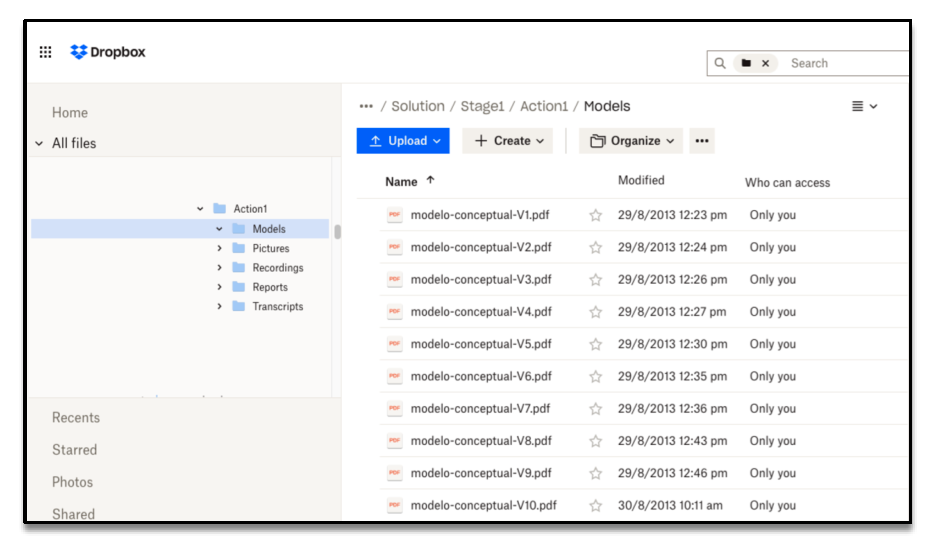
\includegraphics[width=\columnwidth]{images/Intermediate-Products}
	\caption{Repository structure}
	\label{fig-info-study}
\end{figure}

\section{Ethnographic study}\label{sec-reseach-execution}
We report the results of the ethnographic study chronologically. First, we describe the analysis of the RGUS's preferred literature sources and review the RGUS' specific experimental material. Later, we comment on our experiences replicating an existing experiment. Finally, we describe how we formalized the information into concept and process models using interviews, focus groups, and workshops.

\subsection{First Approximation}
In the first stages of the investigation, the researchers did not have an ethnographic methodology in mind but something less demanding, in line with existing qualitative studies, e.g., \cite{Johanssen-2019-Continuous-SE-support}, \cite{Strandberg-2019-Ethical-Interviews-SE}, and \cite{Yang-2021-interview-study-developers}. Accordingly, the researchers conducted interviews to clarify the RGUS knowledge and convert it directly into models. 

The interviews with RGUS members provided only limited public knowledge about experimentation. The experimenters believed that interviews were unnecessary because the researchers could acquire knowledge by studying the literature that the experimenters considered the standard, e.g., \cite{Wohlin-2000-Experimentation-SE}. Hence, we studied the literature, too.

However, communication became problematic when the interviews progressed into specialized areas, such as concrete families of experiments. For example, the experimenters supported their storytelling using specific experimental materials the researchers did not have. Nor did the researchers know to understand the experimenters' discussions. At this point, the need for a different research methodology --ethnography-- became apparent. Consequently, the researchers switched minds and continued at a slower pace. We carried out additional activities to understand the standard literature and experimental material. The interaction with the experimenters also changed. For example, the researchers participated first as experimental subjects and later as team members in one of the RGUS families of experiments.

\subsubsection{Analysis of the relevant literature}
The experimenters use the books by Wohlin \textit{et al.} \cite{Wohlin-2000-Experimentation-SE} and Juristo \& Moreno \cite{Juristo-2001-SE-experimentation} as primary sources for their experimentation process. They also utilize specific papers that advise how to experiment in SE, e.g., Basili \textit{et al.} \cite{Basili-1986-ESE}, and Kitchenham \textit{et al.} \cite{Kitchenham-2002-empirical-research-guidelines-SE}. Basili \textit{et al.}'s work \cite{Basili-1999-families-experiments} was also considered relevant due to the experimenters' interest in carrying out experimental replications.

We reviewed the literature in depth. We noticed that the sources do not use coherent terminology. At the outset, it seemed to the researchers that the literature describes different experimental procedures. They later verified that the different terms refer to essentially the same activities, e.g.:

\begin{itemize}
	\item Wohlin \textit{et al.} \cite{Wohlin-2000-Experimentation-SE}: "Experiment idea, Experiment scoping, Experiment planning, Experiment operation, Analysis \& interpretation, Presentation \& package, and Experiment report."
	\item Juristo \& Moreno \cite{Juristo-2001-SE-experimentation}: "Objective Definition, Design, Execution, and Analysis."
	\item Basili \textit{et al.} \cite{Basili-1986-ESE}: "Definition, Planning, Operation, and Interpretation."
	\item Kitchenham \textit{et al.} \cite{Kitchenham-2002-empirical-research-guidelines-SE}: "Experimental context, Experimental design, Conduct of the experiment and Data Collection, Analysis, Presentation of results, and Interpretation of results."
\end{itemize}

We looked for additional ESE books to verify whether terminological diversity was a widespread problem. We only found a new edition of Wohlin \textit{et al.}'s book \cite {Wohlin-2012-experimentatio-SE}, and the specialized books by Runeson \textit{et al.} \cite{Runenson-2012-case-study-SE} and Kitchenham \textit{et al.} \cite{Kitchenham-2015-Evidence-Based-SE}. As expected, these books share standard terms but use diverse terms throughout the text, contributing to the terminological diversity.

\subsubsection{Review of experimental material}\label{subsubsec-review-experimental-material}
The RGUS' experimental materials are a promising source of information since they represent the work performed during almost two decades of experimentation and reflect the tacit knowledge \cite{Polanyi-1996-tacit-k} present in the group. However, accessing the experimental materials was challenging; materials were scattered and disorganized. We needed the experimenters' help to find specific documents/data files, understand their structure and contents, and gain further access to related materials.

The experimental materials evolve. Experiments vary widely in documentary support, independently of their date. The experimental family explains the differences more significantly than the time; the materials related to different families of experiments show significant differences, e.g., digital raw data versus physical papers written with raw data or automatic tools to measure variables versus manual tools.

Concerning the experimental process, all experimental materials generally describe the activities carried out. The execution order and the relationship between experimental activities are unclear; they rely on the experimenters' tacit knowledge. Terminological diversity also affects experimental materials, especially among families of experiments.

We intended to reflect the RGUS knowledge in process and conceptual models. However, we largely failed to consolidate the terminology, so the resultant model, e.g., see this 
\href{https://zenodo.org/record/7093417#.YyjHb-zMLUI}{\ul{link}}, was relatively simple. However, this abstract preliminary model was satisfactory for continuing the ethnographic research.

\subsection{Becoming active participants}\label{replication}
The concepts acquired by the researchers were uncertain. We needed some external confirmation. We decided to apply the learn-by-doing methodology \cite{mendoza-2019-learn-by-doing-methodology} by experimenting and determining whether our understanding was correct.

\subsubsection{Experiment selection}
Instead of designing an experiment from scratch, the researchers replicated an experiment previously conducted by the RGUS. The replication has been published elsewhere.

Conducting a replication of the experimenters' previous work attracted their attention and guaranteed collaboration. Furthermore, the replication would allow us to recreate the design, execution, analysis, and reporting of an experiment that, until then, we only knew due to the examination of the written materials. Finally, the replication would help us better understand the experimenters' motivations and decisions.

\subsubsection{Replication planning}
Various problems hinder replication \cite{Gallardo-2012-CG-PL-SE}, \cite{Vegas-2006-communication-researchers}, \cite{Miller-2005-replicating-SE-experiments}, \cite{Gomez-2014-understanding-replication}, \cite{Demagalhaes-2015-replications-SE}, \cite{Carver-2010-guidelines-replication-SE}, being the main one the absence of a detailed account of the experimental activities. For example, how to approach the experimental design, which experimental objects are necessary, and in which order. We requested the cooperation of the experimenters who ran the baseline experiment to schedule the experimental activities and adapt the design to the new context where the replication would be run.

\subsubsection{Conduction}
Efra\'in R. Fonseca C. performed a literal replication \cite{Gomez-2014-understanding-replication} in an external academic setting to the RGUS.

The existence of explicit experimental materials such as questionnaires, task descriptions, and programs significantly eased experiment conduction since the researchers defined all relevant aspects in advance. The measurement was the most complex and controversial aspect. Let us say that the experimental subjects return test cases, but these test cases are manually interpreted and not run. The experimenters' cooperation was again needed to complete the measurement. Even if the measurement procedure looked controversial, it made complete sense after discussion. We learned that the experimental protocols depend on the experimental task, which depends on the research area. The remaining steps, e.g., calculating measurements from raw data and formatting, did not imply any uncertainty. It was possible to reproduce the duplicate files used in the baseline experiment.

\subsubsection{Analysis and reporting}
We sought help to analyze and report the replication since we did not have statistical training. In retrospect, both the analysis and the report were simple to perform since the experimental design used (\textit{cross-over}) was associated with a well-defined analysis method \cite{Vegas-2016-crossover-designs-experiments-SE}. On the other hand, there were reporting guidelines available \cite{Carver-2010-guidelines-replication-SE}. The experimenters confirmed that the analysis and reporting of experiments generally do not imply substantial SE challenges.

The differences observed between replication and the baseline experiment confirmed our belief that, at least in the case of the RGUS, there are no clear guidelines that allow literal, external, and independent replication \cite{Gomez-2014-understanding-replication} of the original experiment, irrespective of the existence of incidents in the replication's execution. As a corollary, the original experimenters' presence was necessary to compare the baseline experiment results and replication.

\subsubsection{Assessment}
The replication was, in retrospect, the key to clarifying the RGUS' experimental process. The replication exercise increased the researchers' knowledge and enabled the verification of previous findings, e.g., the RGUS terminology. We made some discoveries, e.g., the specificity of experimental protocols and, notably, the confirmation of extensive tacit knowledge.

\subsection{Modeling the RGUS' knowledge}\label{subsec-conocimiento-grupo}
After the experiment, the researchers were not sure which way to go. The investigation was successful from an operational viewpoint, except for the analysis, which required specific statistical knowledge. The researchers satisfactorily completed all other activities. The models improved somehow during the replication, e.g., see this \href{https://zenodo.org/record/7101676#.YytEquzMLUI}{\ul{link}}, and to the best of our knowledge, we did not overlook anything relevant.

However, we were not completely satisfied with the ethnographic study. We replicated \textbf{one} experiment in \textbf{one} concrete SE area. Still, nothing guaranteed that we would not need the experimenters' help in a hypothetical subsequent replication \cite{Juristo-2012-replication-SE} \cite{Gomez-2014-understanding-replication}. The presence of tacit knowledge represented a severe threat to validity.

\subsubsection{Semi-structured interviews}
We decided to organize a new series of semistructured interviews with the experimenters. The key difference with the first approximation was that we would not discuss the SE experimental process \textit{in general}. Still, we would focus on replicating \textit{specific families of experiments}. Given the experience acquired during the replication, we believed this strategy could expose the tacit experimenters' knowledge.

We created an open-ended questionnaire to motivate the experimenters to give a spontaneous but relatively ordered account of their experiences. We gave up note-taking and captured the interviews with video, including the experimenters' body language. We also collected paper sketches (e.g., see Fig.~\ref{fig-proceso-exp-boseto}) that some experimenters used to support their narrative. We analyzed videos and sketches using protocol analysis \cite{Pressley-1995-verbal-protocols}. We created a report after each interview, e.g., see this \href{https://zenodo.org/record/7102137#.YytgDOzMLUI}{\ul{link}}.

\begin{figure}[htbp!]
	\centering
	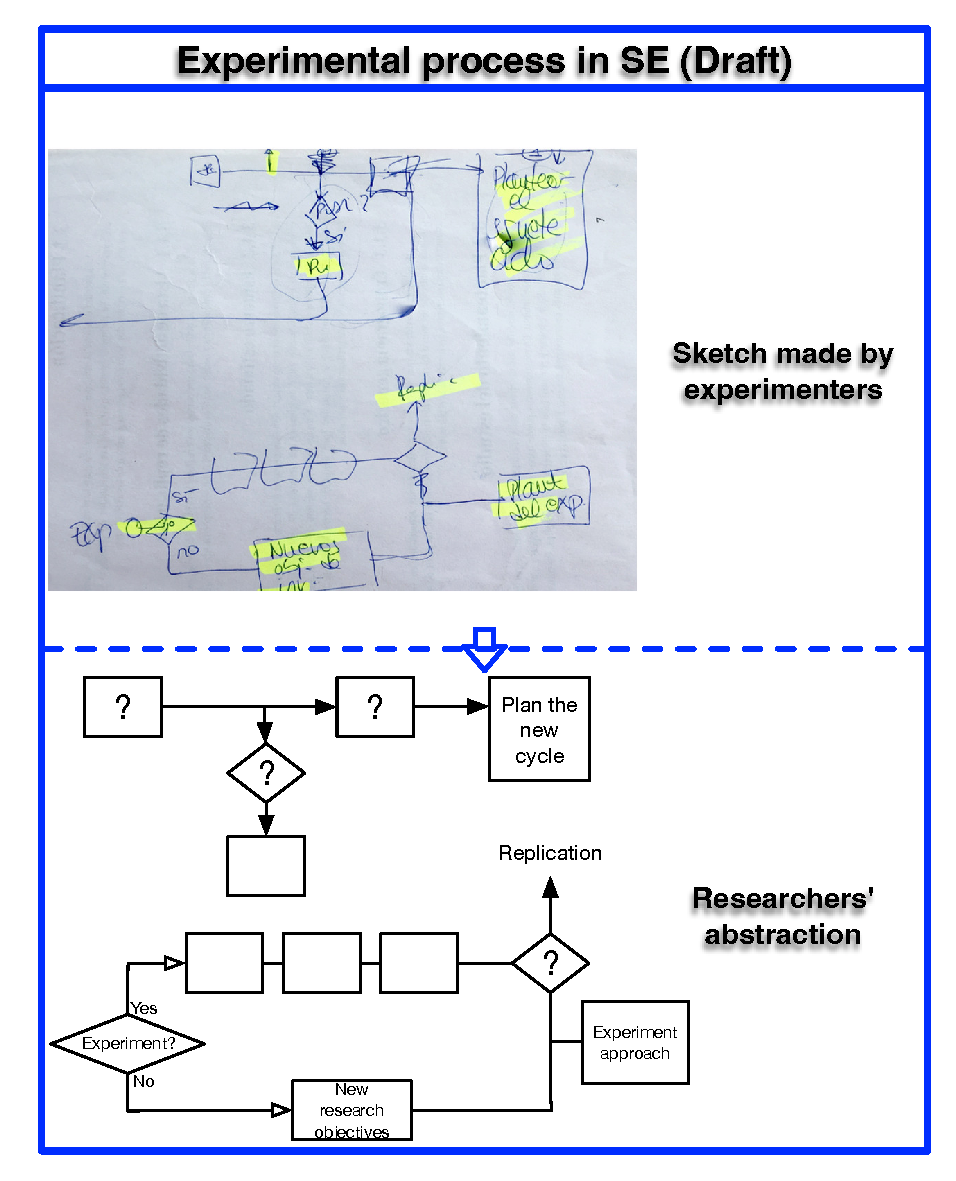
\includegraphics[width=\columnwidth]{images/Process-Approximation-Draft}
	\caption{Example of a sketch made by the experimenters. \added[id=v2]{The researchers have used drafts like this to progress in the definition of the experimental process workflow described in Section~\ref{sec-results:process-workflow}.}}
	\label{fig-proceso-exp-boseto}
	\highlight{This new figure replaces the previous Figure 2, which was included}
	\highlight{in the first version of the manuscript.}
\end{figure}


The process was smooth since each experimenter offered a coherent narrative. We conducted a total of seven interviews with six RGUS members. Each time, we refined the acquired knowledge. The reader can check the models' evolution through this \href{https://zenodo.org/record/7102213#.YytmMezMLUI}{\ul{link}}. When the progress was marginal, the interviews concluded.

\subsubsection{Preliminary models}\label{sec:preliminary-models}
We created process and concept models. We also created a workflow to represent the relations between activities that appeared during the investigation. Please note that we introduce the outstanding characteristics of the models only because the ethnographic research has not ended yet. The models and the workflow have to be validated by the experimenters. We will provide full details in Section~\ref{sec-results}.

\begin{itemize}
	\item \textit{Preliminary} experimental process model: We realized that the RGUS conducts experiments that resemble the processes we use in SE, e.g., ISO/IEC 12207 \cite{ISO-IEC-IEEE-12207}. In the end, they are all processes. Hence, we abstracted six high-level experimental processes: support, generation of pieces of knowledge, publications, synthesis, basic, and organization. Each process has several related activities. For example, the \textit{basic process} includes the activities: pre-execution (context adaptation, experiment redesign, and experiment design), execution (pre-session, in-session, and post-session), and post-execution (raw data generation, data processing, data analysis, and data interpretation) (see this \href{https://zenodo.org/record/7102301#.Yyt0GOzMLUI}{\ul{link}}).
	
\item \textit{Preliminary} workflow: It shows how the connections between experimental processes (see this \href{https://zenodo.org/record/7102360#.Yyt1a-zMLUI}{\ul{link}}). According to the experimenters, the experimental process has three main stages or paths: experimentation, replication, and synthesis. The activities performed in each step can be classified according to the experimental process model described above.

An experimenter does not usually carry out all activities, although they know how to perform them (maybe not flawlessly). In turn, different responsibilities are typically assigned to the same experimenter. We identified the following roles (the names suggest their responsibilities): (1) \textit{Research Manager}, (2) \textit{Experiment Manager}, and (3) \textit{Senior Experimenter}. These roles are responsible for (1) planning the experimental research, (2) managing the logistics, and (3) conducting the experiment in practice, respectively. The study showed overlapping responsibilities among roles, e.g., the domain and topic selection for the experiment.

	\item \textit{Preliminary} conceptual model: Preliminary results at the conceptual model level show activities similar to what the books say, indicating that it has evolved the least (see this \href{https://zenodo.org/record/7102387#.Yyt7W-zMLUI}{\ul{link}}).
\end{itemize}

\subsubsection{Double-checking using focus groups}\label{subsubsec-focus-groups}
Interviews have limitations for eliciting tacit knowledge. When the preliminary models were ready, we made a presentation to all RGUS experimenters for double-checking. 

As we said above, we organized the semistructured interviews around families of experiments. It was a fortunate mistake. The families of experiments are pretty homogeneous. The experimenters involved in the family quickly agree and provide a coherent picture of the experimental process. However, experimenters from different families disagree on many aspects, particularly the specific arrangements used in the experimental families. For instance, the experimenters never agreed on the activities related to the experimental design.

We aimed to solve the disagreements using a consensus-reaching technique, e.g., DELPHI \cite{Dalkey-1967-Delphi}. However, social pressure was not a problem. We decided to organize focus groups. The most senior experimenter led the meetings as a moderator, but only to keep the discussion on track. The researchers only observed. Each session lasted at least two hours. Before the focus group, the experimenters reviewed the concept models. We started with the concept models because they were more straightforward and smaller. The process models/workflow were later updated based on the changes to the concept model.

The focus groups prompted a substantial growth in the models' details after heated discussions that reconfirmed the existence of terminological diversity \textit{even among experimenters who carried out similar activities within the same family of experiments}. The most likely reason seems to be the training that each experimenter received. Talking about "training" in the context of the RGUS is probably incorrect since its members are self-educated, with few exceptions. The preferred SE experimental literature, e.g., \cite{Creswell-2009-Method-Approaches}, \cite{montgomery-2019-Design-Analysis-Experiments}, did not drive self-education. Few of these materials existed when the experimenters started their careers. The experimenters chose the training materials according to their preferences and the experimental families in which they participated. Terminological diversity was the logical consequence.

The experimenters did not reach a consensus during the focus group exercise. The discussions with experimenters of different families exhibited a characteristic circular pattern: An experimenter triggered a change later undone by another. Substantial agreement was only possible \textit{within each family of experiments}. The progress we achieved during the replication phase of the ethnographic research (see Section~\ref {replication}) was possible due to our focus on concrete families of experiments, a fact that we completely ignored at that time.

The concept model that we obtained at this stage appears in this \href{https://zenodo.org/record/7102405#.YyuAfOzMLUI}{\ul{link}}. Notice that the agreement is apparent. 

\subsubsection{Role-focused workshops}\label{subsubsec-focus-groups-role}
We did not aim to explore SE family-specific experimental processes. Albeit enjoyable, we perceived it as future research. We tried to use the limited Ph.D. time to improve the models by switching the perspective from experimental family to \textit{experimental role}. There was no reason to think that roles could contribute to the agreement. However, we used the concept model to drive the focus groups, not the process models. Roles are connected to activities, not concepts. Activities looked more uniform than concepts. It was worth trying.

The strategy was simple. Experimenters who played the same role gathered informally and discussed the tasks associated with that role \textit{only}. Meetings were peaceful (the focus group meetings were less gentle), and the conversations were constructive. Putting aside family-specific issues, we could double-check the existence of roles (the experimenters agreed that roles make sense, even if they have never perceived their responsibilities in these terms). 

We could also break down the conceptual model into role-specific conceptual models. They represent groups of concepts the experimenters use when they play a specific role. Most experimental activities are role-specific, e.g., the senior experimenter role uses the run-kit concept exclusively. The role-specific conceptual models are available through these links: \href{https://zenodo.org/record/7102431#.YyuFvuzMLUI}{\ul{1}}, \href{https://zenodo.org/record/7102450#.YyuG2OzMLUI}{\ul{2}}, \href{https://zenodo.org/record/7102464#.YyuIkOzMLUI}{\ul{3}}.
\section{Results}\label{sec-results}
The ethnographic research yielded three main results: (1) an \textit{experimental process workflow}, (2) an \textit{experimental research concept model}, and to a lesser extent, (3) an \textit{experimental process model}. They are described below. We have not used standard notations, e.g., UML or BPMN because experimental researchers (and probably readers) have different ages, backgrounds, and careers. We have valued the communication above model formality.

\subsection{Experimental process workflow}\label{sec-results:process-workflow}

The so-called \textit{experimental process workflow} (EPW) represents the tasks carried out during SE experimentation (according to the RGUS' perspective) and their logical sequence. The workflow is available in this \href{https://zenodo.org/record/7102486#.YyuKruzMLUI}{\ul{link}} and, with lower resolution, it is shown in Fig.~\ref{fig-EPM-construction}.

The EPW model shows three well-defined paths corresponding to the key SE experimental research processes: (1) Experimentation (purple), (2) replication (green), and (3) synthesis (yellow). In addition, based on the existence (or not) of new moderator variables and new knowledge generated in the last round, there are activities of analysis associated with planning new cycles of experimentation, replication, or synthesis and reporting related to the publication of results, respectively (highlighted in blue). Such processes appear associated with the experimentation and synthesis paths.

\subsubsection{Experimentation path}
Experimentation is the heart of experimental research since replication and synthesis stem from it. However, in some circumstances, experimentation may require the previous execution of the synthesis (e.g., when choosing the topic of the experiment) or replication (e.g., in adaptation to the context) activities. According to the experimenters, the experimentation activities are:
\begin{itemize}
	\item Selecting the experiment domain.
	\item Selecting the experiment topic.
	\item Selecting the experimental hypothesis.
	\item Planning the experiment.
	\item Creating the experimental kit.
	\item Executing and postexecution of the experiment.
\end{itemize}

When the experiment results do not meet the experimenters' expectations, they plan a new cycle of experimental research redesigning and conducting the experiment again. This redesign activity usually happens when investigating fundamental topics.

\subsubsection{Replication path}
Replication is the practice on which scientific knowledge is based, hand in hand with the synthesis of results \cite{Roizer-2014-reproducibility}. The RGUS agrees that replication is essential for experimental research both explicitly (RUGS' experimenters claim that) and, more importantly, implicitly (the experimental workflow contains minute details about replication activities). The replication path consists of the following activities:

\begin{itemize}
	\item Definition of replication.
	\item Study and update the experimental kit.
	\item Adaptation to the context, and
	\item Creation of operational elements.
\end{itemize}

\subsubsection{Synthesis path} 
According to the RGUS' experimenters, results can be synthesized from systematic literature reviews, systematic mapping studies, or experiments sharing a common goal (a family of experiments). In each case, the experimenters apply particular synthesis techniques (e.g., aggregated or individual patient meta-analysis) and interpret the results. During the interpretation, the researchers can identify moderator variables or generalize pieces of knowledge. Such findings may lead to reforming the synthesis' goals or conducting a new cycle of experimental research. In addition, the experimenters generally publish results after a synthesis, hand in hand with planning the next round.

The information obtained from the RGUS looks quite general and in line with the community's understanding of synthesis. That is correct. Our findings are somewhat predictable because the RGUS had no experimenters with the required expert knowledge available during this research. On the other hand, the limited insight into synthesis probably represents an indirect confirmation of the ethnographic research's success. Our understanding goes in proportion to the expert knowledge available, and there is much-specialized knowledge on the RGUS about experimentation and replication, which was our primary goal. 

\subsection{Experimental research concept model}
This research's conceptual model is not monolithic; on the contrary, it is composed of three submodels (more accurately, viewpoints) aligned with prominent experimental roles (research manager - RM, experiment manager - EM, and senior experimenter - SrEx). The activities described in the EPW lead to such views. The experimenters took into account the best-known generic phases of the experimentation process to develop new versions of the conceptual model (starting from version eight, generated in the first phase of the interviews; see \href{https://zenodo.org/record/7102387#.Yyt7W-zMLUI}{\ul{link}}).

\subsubsection{Research manager (RM) viewpoint}
The RM viewpoint is available in this \href{https://zenodo.org/record/7102431#.Yyxi1ezMLUJ}{\ul{link}}. The RM has the following perspectives:
\begin{itemize}
	\item In the experiment definition phase, the RM manages the "problem definition" and the "hypothesis definition." 
	\item During the experiment design phase, the RM takes care of the "human resource management" that could "run," "replicate," or be interested in "replicating" the experiment. In addition, the RM receives information regarding the "Expected results," "Execution context," and "new variables of interest."
	\item While the experiment runs, the RM monitors events. However, the data acquisition phase is transparent to her.
	\item During the data analysis phase, the RM learns the "analysis results" and contributes to the definition of "findings," "publications," and "pieces of knowledge."
\end{itemize}

\subsubsection{Experiment manager (EM) viewpoint}
The EM viewpoint is available in this \href{https://zenodo.org/record/7102450#.YyxjmezMLUJ}{\ul{link}}. The perspective is as follows:

\begin{itemize}
	\item In the experiment definition phase, the EM actively interacts with all experiment entities, hand in hand with the Senior Experimenter (SrEx). However, in the "hypothesis definition," the EM is only an observer.
	\item In the experiment design phase, the EM focuses on improving the "experiment guides" regarding "instruments," "objects," and the "experimental kit." Additionally, the EM can analyze the context in which the experiment occurs.
	\item During the experiment execution and data acquisition phases, the EM does not lose sight of the "events" that arise and could affect the results. The EM also analyzes the "correctness" of the "collected items" and the "raw data."
	\item In the data analysis phase, the EM cooperates with the "re-analysis" in search of new "variables of interest" to the RGUS. Additionally, the EM can observe the analysis results to suggest findings that could be useful in publications.
\end{itemize}

\subsubsection{Senior experimenter (SrEx) viewpoint}
The SrEx viewpoint is available in this \href{https://zenodo.org/record/7102464#.Yyxl4ezMLUJ}{\ul{link}}. The perspective is as follows:

\begin{itemize}
	\item In the experiment definition phase, the SrEx observes the "experiment definition," hypotheses' "levels," and "metrics" in the first phase of the experimental investigation. The SrEx participates in the definition of the "hypothesis," "factors," and  "response variable."
	\item In the experimental design phase, the SrEx interacts with a large number of entities; hence, it is necessary to divide such a phase into three subphases for this role: \textit{experimental operation design}, \textit{experiment design}, and \textit{artifact generation}.
    \begin{itemize}
	    \item During the \textit{experimental operation design}, the SrEx defines the "experimental objects" for each "experimental task," considering the minute details of each experimental object's characteristics.
	    \item During the \textit{experiment design} proper, the SrEx establishes the execution context's "parameters," the "design type" with its "groups" and assigned "experimental subjects," the "levels" defined and their combination per "session" and "period," "experimental instruments," and the "measurement procedure." 
        \item Finally, in the \textit{artifact generation}, the SrEx fundamentally develops the "run-kit," which includes the construction of the instances of "guides," "experimental instruments," and "experimental objects." Such "instances" are the tools that the "subjects" need to participate in the "experiment."
	\end{itemize}
	\item While the experiment runs, the SrEx records all the events produced to analyze their impact on the experiment results.
	\item During data acquisition, the SrEx records the resulting collected items, creates the raw data, and obtains measurements.
	\item Finally, in the data analysis phase, the SrEx performs the analysis, obtains the findings, and prepares the publications with the RM and EM's help.
\end{itemize}

\subsection{Experimental process model}
The workflow and the conceptual models represent the experimental research process carried out in the RGUS. Other experimental research groups may work differently. We have created an initial (generic, i.e., generally applicable) experimental process model (EPM) with the help of the most experienced experimenter at RGUS. The software life cycle inspired the model \cite{ISO-IEC-IEEE-12207}. We have adapted the concepts used in the ISO/IEC 12207 to the SE experimentation realm. Most items have been taken from the EPW (see Figure \ref{fig-EPM-construction}); a lesser portion derives from the conceptual models. The complete process model can be obtained in this \href{https://zenodo.org/record/7105096#.YyxoCOzMLUI}{\ul{link}}.

The EPM contains six groups of processes that define the SE experimental research life cycle: (1) the Basic process, (2) the Support process, (3) the Knowledge item generation process, (4) the Publication process, (5) Synthesis process, and (6) Organizational process. 

\subsubsection{Basic process}
The basic process involves fundamental activities performed by the experimenters as RM, SrEx, and EM roles before, during, and after running an experiment. Before the experiment, the activities focused on its design, e.g., adapting the experiment to the research context. During the experiment, experimenters pay attention to, e.g., the events that occur before, during, and after the experiment's execution session. The activities performed after the execution focus on the data, e.g., generating raw data and data analysis.

\subsubsection{Support process}
The support process includes activities that the EM performs to manage the materials and support those interested in performing replications, such as:

\begin{itemize}
	\item The management of materials before the experiment's execution (e.g., experiment design document), 
	\item The materials used during the experiment (e.g., templates for data collection), 
	\item The materials obtained at the end of the experiment (e.g., filled templates and subjects' code.), and
	\item Knowledge transference as a support style during replication activities.
\end{itemize}

\subsubsection{Knowledge items generation process}
The knowledge items generation process consolidates the activities carried out by the RM to manage the knowledge acquired after each experiment, e.g., the knowledge generated in each experimentation phase, the knowledge transferred to professionals, or the knowledge generated during the identification of moderator variables.
   
\subsubsection{Publications process}
This group of activities focuses on reporting the experiment findings (led by the SrEx), aggregation of results (by the EM), and experimentation goals (by the RM).

\subsubsection{Synthesis process}
The EM carries out the synthesis processes. Different types of synthesis have different evidential levels, e.g., meta-analysis, re-analysis, and informal aggregation.

\subsubsection{Organizational process}
The organizational process includes RM's management activities over the SE experimental research cycle, e.g., human resources and publications management. Likewise, the EM also performs management activities on the experiment materials. Finally, some activities related to synthesis management have not been assigned to any role yet.

\begin{figure*}[htbp]
\begin{center}
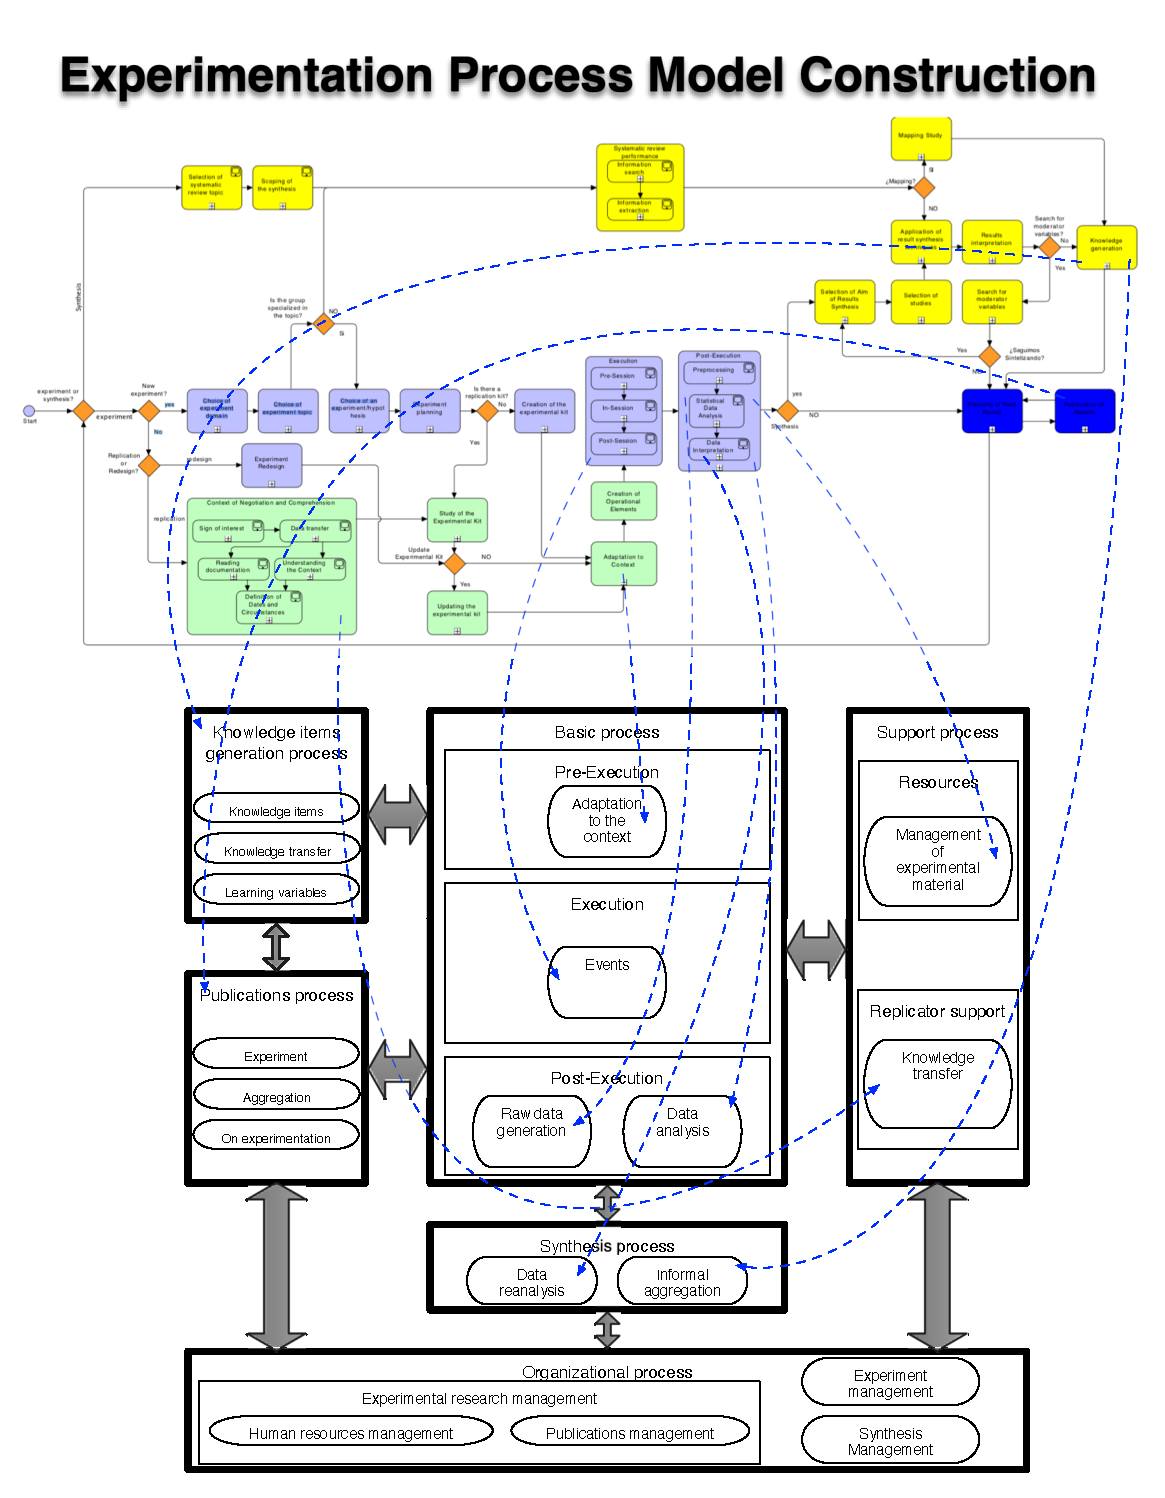
\includegraphics[trim=0 0 0 48,clip,width=0.95\textwidth]{images/Experimentation-Process-Model-Construction}
\caption{Relationships between the \textit{experimental process workflow} (top) and the \textit{experimental process model} (down).}
\label{fig-EPM-construction}
\end{center}
\end{figure*}

Figure \ref{fig-EPM-construction} shows a not-very-good coincidence between the activities of the EPW and those of the EPM since, as indicated before, each model has its purpose; still, we found several relationships.

This model is plausible but based on the RGUS' perspective alone. Further research (in this regard, see Section~\ref{sec-conclusions}) is necessary to ensure that the model represents the experimental SE community's experimental process.
\section{Discussion and related work}\label{sec-related}
This research aims to find out how experimenters work in practice. After conducting the ethnographic research, we obtained models (process, workflow, and conceptual). The conceptual model connects with empirical researchers' "prominent picture" of their research area. The process and workflow models represent a novel contribution; to our knowledge, such detailed descriptions of the experimental process are unavailable in the existing literature.

The models described in Section~\ref{sec-results} are available in full detail online. In this section, we would like to focus on some interesting model features:

\begin{itemize}
	\item \textbf{The experimental process is broader} than we usually recognize as "experimentation". An experiment can be characterized as a small (or not that small) research project. It includes activities related to (see this \href{https://zenodo.org/record/7105096#.YyxsxezMLUJ}{\ul{link}}):
		\begin{itemize}
			\item management (resources, research lines, among others.),
			\item negotiation (e.g., with companies), 
			\item document/artifact support, 
			\item publication, among others.
		\end{itemize}
Although all empirical researchers know these activities, it is surprising that they are seldom mentioned (if ever) in ESE literature. To the best of our knowledge, reference texts, e.g., \cite{Wohlin-2000-Experimentation-SE}, \cite{Juristo-2001-SE-experimentation}, \textbf{do not address these activities beyond marginal notes}. Such richness in the number and diversity of activities raises obvious consequences in experimental education and training.
	\item The ethnographic study revealed one consequence of such diversity. It is possible, albeit unlikely, that one experimenter performs all experimental activities. These activities are not only complex: they demand time. In a project (research or not), the diversity of activities is usually associated with roles with well-defined responsibilities. \textbf{Also in experimentation. We identified three roles}: (1) \textit{Research Manager}, (2) \textit{Experiment Manager}, and (3) \textit{Senior Experimenter}. These roles are probably related to the RGUS' size; smaller (or larger) groups may have more generic/specialized roles. The concept of~\textquotedblleft role\textquotedblright~applied to experimentation is unusual but not entirely new. Mohamed \textit{et al.} \cite{Mohamed-1993-roles-ESE} proposed a framework to conduct ESE experiments. This framework was based on a merge between statistical and SE process concepts, \textbf{including explicit roles}.
	\item The high-level conceptual model (see this \href{https://zenodo.org/record/7102405#.YyxvFOzMLUK}{\ul{link}}) could be endorsed by any experimenter (with some complaints depending on their specialization area, as it happened during the ethnography). However, when the concept of a role appears in the scene, the high-level model is just \textbf{an abstraction of the information handled by the roles}. In other words: the high-level model is incomplete from the roles' viewpoint and thus partially valid. The high-level model evokes the viewpoint of the \textit{senior experimenter} (see this \href{https://zenodo.org/record/7102464#.YyxvsezMLUK}{\ul{link}}), but with fewer details. In turn, the \textit{experiment manager} (see this \href{https://zenodo.org/record/7102450#.Yyxv6ezMLUL}{\ul{link}}), and the \textit{research manager} (see this \href{https://zenodo.org/record/7102431#.YyxwGezMLUL}{\ul{link}}) pay little attention to the design and execution details because the \textit{senior experimenter} takes care of that. Likewise, the \textit{experiment manager} is not affected by the experimental research in its global context, e.g., collaboration with other groups and replication. Such a concern fits the \textit{research manager}'s role. 
\item We deliberately built the models (process, workflow, and conceptual) to offer a coherent picture. However, as we indicated in Section~\ref{subsubsec-focus-groups}, we could not address the existence of different families of experiments. When experimenters working in other families get together, the models automatically diverge. Therefore, the models represent the maximum achievable consensus obtained during the role-oriented meetings. We are conscious that \textbf{further research is necessary at the family level to discover the peculiarities of each research area}. Such an inquiry could have an impact on the SE community. 
\item The replication problem is related to knowledge transfer \cite{Shull-2004-Knowledge-sharing-issues-SE}. Nevertheless, we wonder what exactly does it mean to transfer knowledge? To what extent or how should it be done? For example, Ferreira \textit{et al.} \cite{Ferreira-2017-planning-experiments} emphasize methodological consistency over discussing methods and techniques. 

There is, apparently, an underlying dichotomy between theory and practice. In theory, formal guides, e.g., replication packages, should describe the process. However, the practice shows that such mechanisms cannot cope with the existing diversity of experimental protocols. The replication process will likely benefit from the specialized, fine-grained knowledge \textbf{at the family level}.
\end{itemize}

The models (process, workflow, and conceptual) and the ethnographic experience have generated some SE experimental process' differential characteristics or viewpoints, e.g., context adaptation and iterative improvement. Previous research pointed out some of these characteristics, e.g., \cite{Mohamed-1993-roles-ESE}, \cite{Sjoberg-2005-survey-experiments-SE}, \cite{Shull-2004-Knowledge-sharing-issues-SE}. We do not wish to provide a detailed account of these differential characteristics herein; that would require a publication of a different character. Instead, we aimed to observe how experimenters work and found out that they perform tasks other than those portrayed in textbooks. \textbf{This is our essential contribution}.

We also know that models represent \textbf{the point of view of a single experimental research group}. We must extend the inquiry to other experimental research groups, ideally to large portions of the ESE community, and check whether they reveal similar behavior patterns.
\section{Threats to Validity}\label{sec-threats}
Validity is the degree to which the research is conducted transparently and without biases. We have followed Runeson et al.'s recommendations \cite[p. 71–73]{Runenson-2012-case-study-SE} to design the ethnographic research and describe the threats to validity. Runeson et al., following Yin \cite{Yin-2009-case-study}, classify threats into four groups: (1) construct validity, (2) internal validity, (3) external validity, and (4) reliability.

\subsection{Construct validity}
Construct validity deals with the degree of agreement between the study constructs, i.e., what the ethnographic researchers have in mind, and the observations made in the field. For example, if the interview questions are not interpreted the same way by the researcher and the experimenters, there is a threat to construct validity. 

The ethnographic method is particularly suitable to oppose this threat because knowledge acquisition progresses gradually. On top of that, we used several techniques during the research to create constructs, e.g., reading, observation, and interviews, among others. The different approaches increase the chances of identifying or solving misunderstandings between the researchers and the RGUS. Using reliable information sources, e.g., standard literature and the RGUS' experimental material, we also prevented construct validity threats. 

Finally, the constructs were validated iteratively by experimenters and researchers during the research project lifespan.

\subsection{Internal validity}
Internal validity addresses the credibility of the causal relationships found during the research. However, this threat does not apply to this ethnographic study, as we do not aim to identify causal relationships but, at most, correlations between phenomena, e.g., when we claim that the number and diversity of experimental tasks explain the existence of roles. Furthermore, most of the findings we provide are descriptive, e.g., disagreements among experimenters of different experimental families.

\subsection{External Validity}
External validity represents the degree of certainty of the findings obtained in an investigation being generalizable, i.e., applied to different contexts of their origin. This threat is prominent in this study since it was carried out in a single instance (an experimental research group) of the population under study (SE research groups that apply empirical methods). As a countermeasure, we chose a highly representative experimental research group.

\subsection{Reliability}
The reliability of a study is the ease with which the research activities and the results obtained can be reproduced by other studies that apply the same methodology in the same RGUS (more likely, in similar experimental research groups). 

As mitigation measures, we have followed the research methodology outlined in Section~\ref{sec-research-method} closely to ensure the reliability of this research. Moreover, we have disclosed all intermediate and final results in a repository available under request to guarantee transparency in the investigation.
\section{Conclusions}\label{sec-conclusions}
Experimental researchers know that experimentation, as described in textbooks and articles, is only an approximation to the daily work in the labs and the field. This study shows the deviations found in a concrete experimental research group. Such divergences do not seem arbitrary but necessary from a systemic viewpoint, e.g., each people have distinct abilities and perform different tasks in a research project.

We do not claim that our findings are commonplace in the empirical community. They may be particular to the experimental research group in which we performed the ethnographic study. However, some clues evidence that peculiar behaviors are usual in the labs and the field. For instance, natural sciences researchers have complained about the replication problem \cite{hines2014sorting}. At least in the sciences (maybe not in SE), replication frequently fails due to experimental setup and conduction changes. These changes are motivated by the researchers' tacit knowledge \cite{Polanyi-1996-tacit-k} \cite{Shull-2002-replicating-SE-experiments-tacit-k}, and consequently, protocols or experiment reports do not declare such changes. Experiment variations happen so frequently that some disciplines coined a (comic) term: \textquotedblleft lab mythology \textquotedblright~\cite{ruben2011experimental} \cite{loukides2015beyond}. Our study has shown that such tacit knowledge is present in SE and manifests at a relatively superficial level, e.g., when researchers from different experimental families discuss their mental models.

Furthermore, anecdotic evidence, e.g., conversations with colleagues, suggests that this "lab mythology" can also be somewhat present in SE. We all know that the experiment reports do not reflect the experimental process precisely. It does not mean experimenters cheat. We all know from experience that some practices work and others do not, and we apply them as required.

We believe that the "lab mythology" is worth studying. If the differential characteristics of the theoretical vs. actual experiment process are research-group specific, the inquiry will end. However, it is also possible that widespread patterns of behavior show up. Bringing such knowledge to the foreground could contribute to the improvement of experimental practice.

We are aware that the findings of this study correspond to the particular perspective of an experimental research group, albeit representative of the ESE community. Therefore, it is necessary to carry out further studies to generalize the results of the present work. We have completed a survey exploring some issues, e.g., terminological diversity, that surfaced during the ethnography. We have also completed a comparative study of the experimental process between the SE and an established engineering discipline. Both works will likely be published shortly. In addition, we plan to conduct more studies (probably not ethnographic, because they require too much time) on this topic soon.
%\section{Data Availability Statements}\label{sec-data-availability-statements}
The data supporting this study's findings are partially available from the links specified throughout the manuscript. Still, restrictions apply to the availability of the whole data due to personal information included. However, the complete data could be available with the authors' permission upon a reasonable request.
%%%%%%% End Content %%%%%%%%%

\section*{Acknowledgment}
This work was supported by the \deleted[id=v3]{project} \replaced[id=v3]{grant PID2022-137846NB-I00 funded by MCIN/AEI/10.13039/501100011033, and by ''ERDF A way of making Europe''}{PGC2018-097265-B-I00 funded by the Spanish Ministry of Science and Innovation and co-financed by FEDER}, and the Universidad de las Fuerzas Armadas - ESPE's Grupo de Investigación en Modelos de Producción de Software e Industria Inteligente (GrIMPSoftII). This work's preprint has been published \cite{Fonseca-2023-experimentation-proccess-SE-unpublished}.

% can use a bibliography generated by BibTeX as a .bbl file
% BibTeX documentation can be easily obtained at:
% http://www.ctan.org/tex-archive/biblio/bibtex/contrib/doc/

\Urlmuskip=0mu plus 1mu\relax
\bibliographystyle{iet}
\bibliography{bibliography}

\appendices
\section{Acronyms}

\begin{table}[h]
	\caption{Acronyms used in the manuscript}
	\label{table}
	\setlength{\tabcolsep}{3pt}
	\begin{tabular}{|p{25pt}|p{115pt}|p{25pt}|}
	\hline
	Item & Term & Acronym\\
	\hline
	1 & Empirical Software Engineering & ESE\\
	\hline
	2 & Research Group Under Study & RGUS\\
	\hline
	3 & Grupo de Investigación en Modelos de Producción de Software e Industria Inteligente & GrIMPSoftII\\
	\hline
	4 & Research Manager & RM\\
	\hline
	5 & Experiment Manager & EM\\
	\hline
	6 & Senior Experimenter & SrEx\\
	\hline
	7 & Experimental Process Model & EPM\\
	\hline
	8 & Experimental Process Workflow & EPW\\
	\hline
	\multicolumn{3}{p{251pt}}{These acronyms have been used throughout the manuscript.}\\
	\end{tabular}
	\label{tab1}
\end{table}


\end{document}
